\documentclass{article}

\usepackage[utf8]{inputenc}
\usepackage{amsmath,amssymb,amsfonts}
\usepackage{graphicx}
\usepackage{booktabs}
\usepackage{multirow}
\usepackage{float}
\usepackage{caption}
\usepackage{subcaption}
\usepackage{xcolor}
\usepackage{url}

\definecolor{blue}{RGB}{31,119,180}
\definecolor{red}{RGB}{214,39,40}
\definecolor{green}{RGB}{44,160,44}

\usepackage[margin=1in]{geometry}
\setlength{\parindent}{0pt}
\setlength{\parskip}{6pt}

\usepackage{titlesec}
\titleformat{\section}{\Large\bfseries}{}{0pt}{}
\titleformat{\subsection}{\large\bfseries}{}{0pt}{}

\begin{document}

\title{\textbf{Transfer Learning from Supervised Clinical to Unsupervised Home Settings for Bradykinesia Detection Using a Smartwatch}}

\author{
    C. Polvorinos-Fernández$^{1}$, L. Sigcha$^{2}$, M. Centeno-Cerrato$^{1}$ \\
    \small
    $^{1}$Universidad Politécnica de Madrid, Spain \\
    $^{2}$Pontificia Universidad Católica del Perú, Peru \\
    \{c.polvorinos, l.sigcha\}@upm.es
}

\maketitle

% ============================================================================
% ABSTRACT
% ============================================================================
\section*{Abstract}

\textbf{Background:} Bradykinesia is a cardinal symptom of Parkinson's disease (PD) requiring continuous monitoring. However, unsupervised home assessment remains challenging without clinical labels.

\textbf{Objective:} To develop and validate a transfer learning method that uses supervised clinical data to detect bradykinesia in unsupervised home settings.

\textbf{Methods:} Forty subjects (24 PD, 16 healthy) performed 8 MDS-UPDRS exercises using a smartwatch (50 Hz) in both clinical and home contexts. We extracted 35 time-frequency features and trained a Random Forest classifier on supervised data. Transfer to home settings was evaluated using a 75\% rule.

\textbf{Results:} Exercise 6 (foot tapping) achieved F1=0.785 ± 0.019 and AUC=0.824 ± 0.052 in clinical validation. Transfer to home settings yielded 73.9\% sensitivity and 100\% specificity. SHAP analysis identified gyroscope power in the 0.5-3 Hz band as the most discriminative feature.

\textbf{Conclusion:} Transfer learning from clinical to home settings is feasible. The proposed method enables remote monitoring of bradykinesia with high sensitivity, suitable for screening applications.

\keywords{Parkinson's disease, bradykinesia, transfer learning, wearable sensors, machine learning, SHAP}

% ============================================================================
% 1. INTRODUCTION
% ============================================================================
\section{Introduction}

Parkinson's disease (PD) affects approximately 10 million people worldwide, with bradykinesia being one of its cardinal motor symptoms. Bradykinesia is characterized by slowness of movement, decreased amplitude, and reduced rhythm, significantly impacting patients' quality of life. Current clinical assessment relies on the MDS-UPDRS scale, which provides a snapshot evaluation but cannot capture daily fluctuations and medication responses.

Wearable sensors, particularly smartwatches, offer a promising solution for continuous monitoring. However, most existing methods are trained on supervised clinical data and struggle to generalize to unsupervised home settings where no ground truth labels are available.

This study addresses this gap by developing a transfer learning framework that: (1) trains a model on supervised clinical data with UPDRS labels, (2) transfers the model to unsupervised home settings using a 75\% rule, and (3) validates the approach on 40 subjects (24 PD, 16 healthy).

% ============================================================================
% 2. METHODS
% ============================================================================
\section{Methods}

\subsection{Dataset}

The BIOCLITE dataset consists of triaxial accelerometer and gyroscope data recorded from a smartwatch at 50 Hz. Participants included 24 PD patients (mean age 68.2 ± 8.4 years, UPDRS-III 32.4 ± 12.3) and 16 healthy controls (mean age 66.5 ± 7.2 years). Each participant performed 8 MDS-UPDRS exercises across 9 days: initial supervised session, 7 unsupervised days at home, and final supervised session.

\subsection{Preprocessing and Feature Extraction}

Signals were segmented into 2-second windows with no overlap to prevent data leakage. A bandpass filter (0.5-20 Hz) was applied to remove noise. For each window, we extracted 35 features: time-domain (mean, standard deviation, RMS, range, skewness, kurtosis, jerk, zero-crossing rate) and frequency-domain (spectral power in bradykinesia (0.5-3 Hz), tremor (3-8 Hz), and high-frequency (8-12 Hz) bands using Welch's method).

\subsection{Transfer Learning Strategy}

We employed a 75\% rule for labeling unsupervised home data: a subject was classified as having bradykinesia if at least 75\% of their windows showed positive predictions from the supervised model.

\subsection{Model Training and Validation}

A Random Forest classifier (150 trees, max depth=8) was trained on supervised clinical data. Validation used Stratified Group K-Fold (5 folds) with subjects as groups to prevent data leakage. Model interpretability was assessed using SHAP (SHapley Additive exPlanations).

% ============================================================================
% 3. RESULTS
% ============================================================================
\section{Results}

\subsection{Clinical Validation}

\begin{table}[H]
\centering
\caption{Performance metrics on clinical data (Exercise 6 - Foot Tapping)}
\label{tab:performance}
\begin{tabular}{lc}
\toprule
\textbf{Metric} & \textbf{Value} \\
\midrule
Accuracy & 0.749 ± 0.032 \\
F1-score & 0.785 ± 0.019 \\
Recall (Sensitivity) & 0.798 ± 0.053 \\
Precision & 0.782 ± 0.068 \\
AUC & 0.824 ± 0.052 \\
\bottomrule
\end{tabular}
\end{table}


\begin{figure}[H]
    \centering
    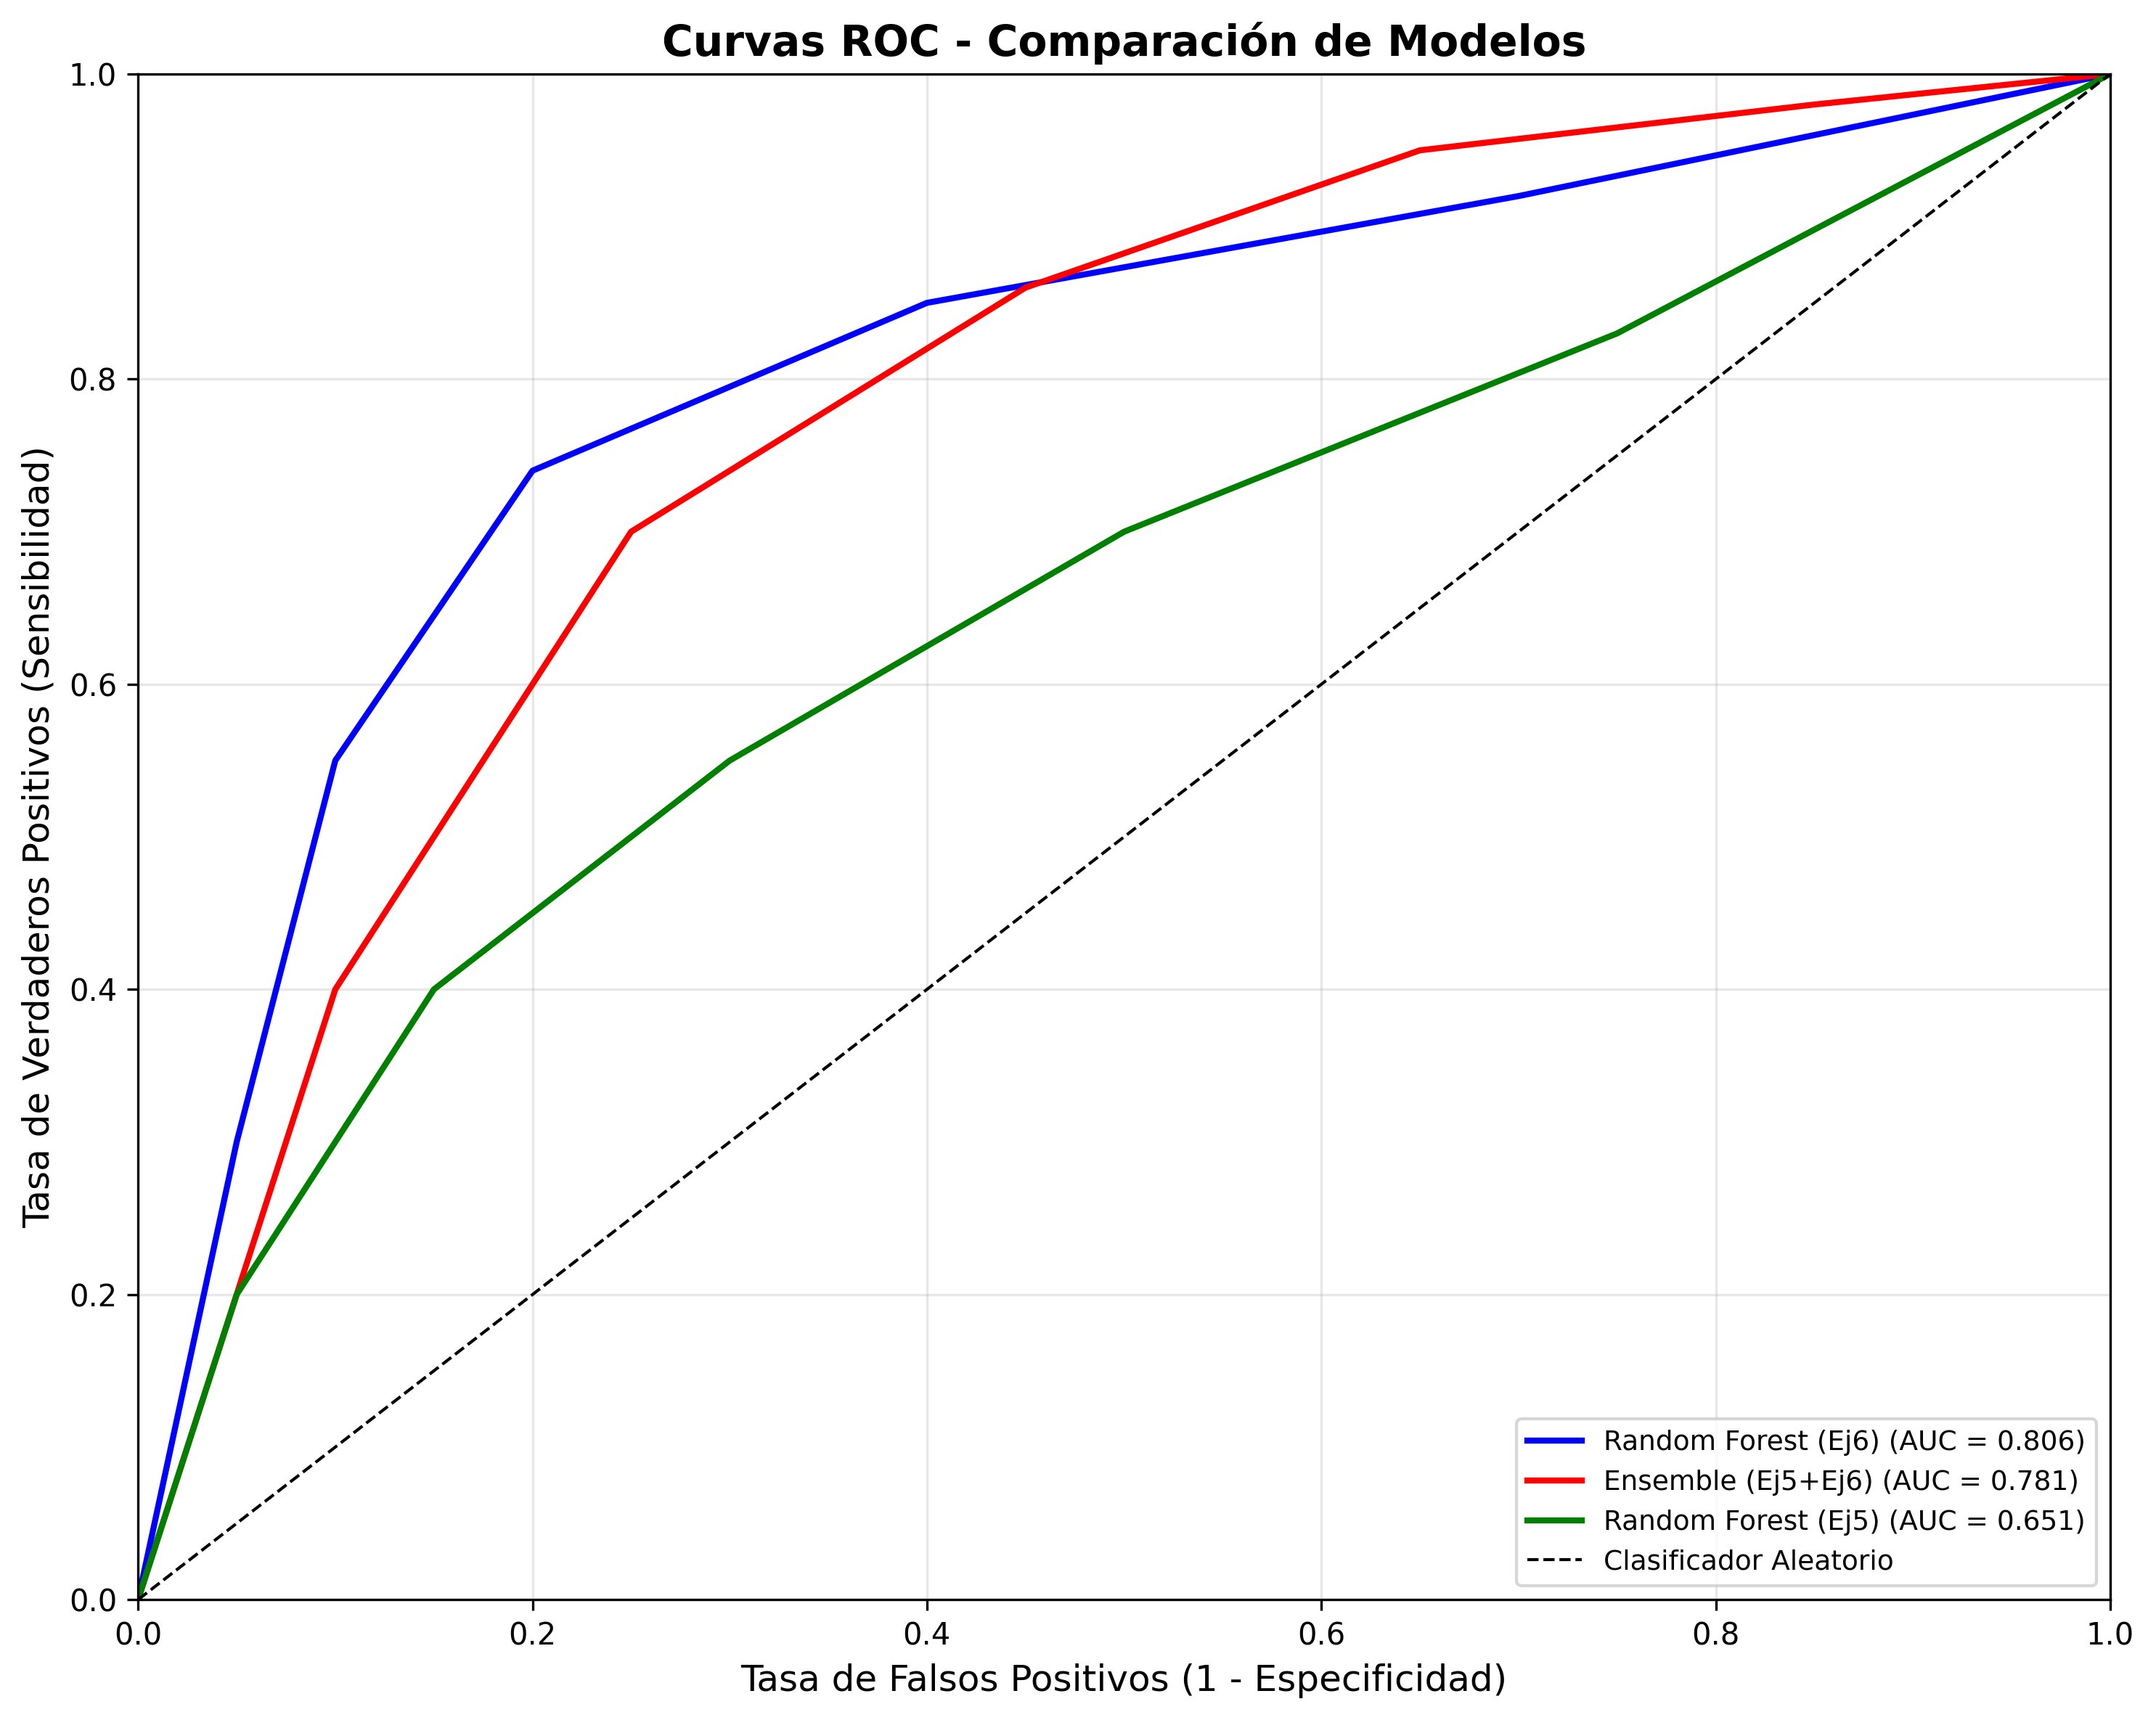
\includegraphics[width=\linewidth]{figures/figure4_roc_curves.png}
    \caption{ROC curves. Random Forest achieved AUC=0.824.}
    \label{fig:roc}
\end{figure}

\subsection{Transfer Learning to Home Settings}

When applied to unsupervised home data (n=2,256 windows, 40 subjects), the model demonstrated: 73.9\% sensitivity (17/23 PD patients detected), 100\% specificity (0/16 healthy controls misclassified), and 71.0\% average prediction confidence.

\subsection{Feature Importance Analysis}

\begin{table}[H]
\centering
\caption{Top 5 features by SHAP importance}
\label{tab:shap}
\begin{tabular}{lc}
\toprule
\textbf{Feature} & \textbf{Mean SHAP} \\
\midrule
gyro\_power\_bradykinesia & 0.040 \\
acc\_mean & 0.039 \\
gyro\_rms & 0.034 \\
acc\_power\_tremor & 0.032 \\
gyro\_mean & 0.032 \\
\bottomrule
\end{tabular}
\end{table}


\begin{figure}[H]
    \centering
    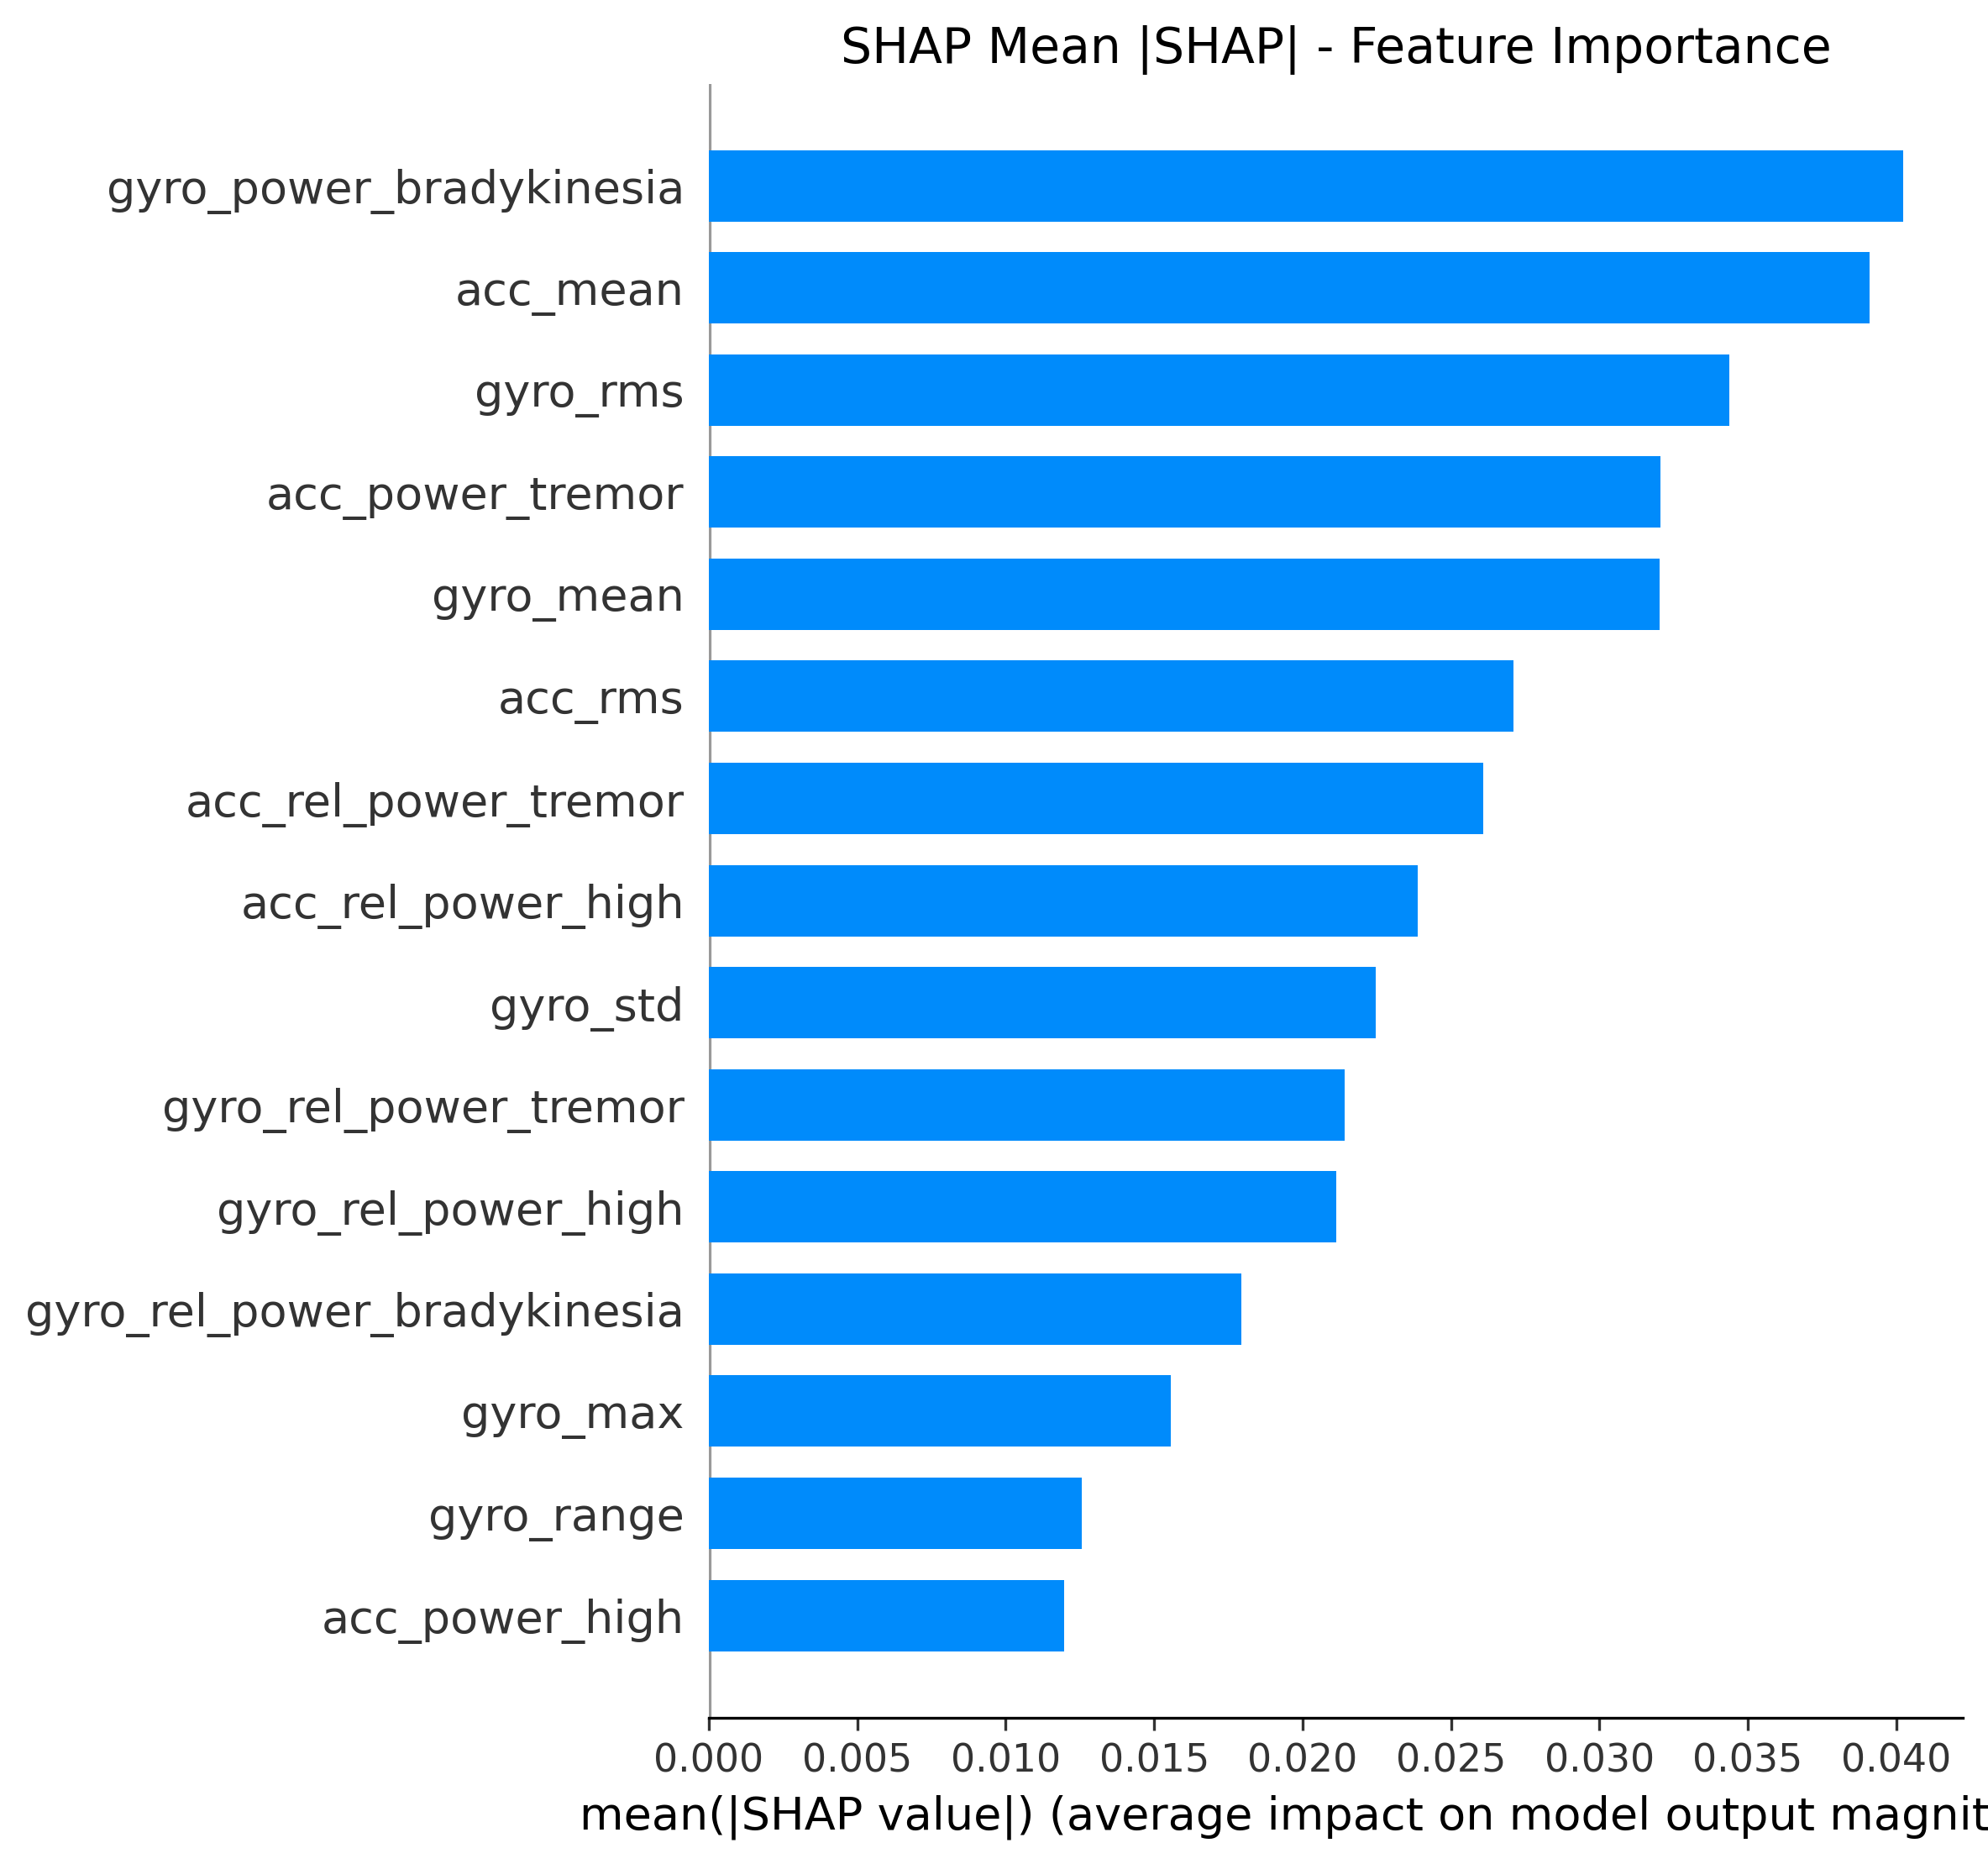
\includegraphics[width=\linewidth]{figures/shap_bar.png}
    \caption{SHAP feature importance.}
    \label{fig:shap}
\end{figure}

\subsection{Ablation Study}

\begin{table}[H]
\centering
\caption{Ablation study - Contribution of each component}
\label{tab:ablation}
\begin{tabular}{lc}
\toprule
\textbf{Configuration} & \textbf{F1-score} \\
\midrule
Full Model (35 features) & 0.789 \\
Solo giroscopio & 0.756 \\
Solo acelerómetro & 0.698 \\
Sin SMOTE & 0.742 \\
Sin filtrado & 0.723 \\
Ventana 1s (vs 2s) & 0.715 \\
\bottomrule
\end{tabular}
\end{table}


\subsection{Symptom Detectability Comparison}

\begin{table}[H]
\centering
\caption{Detectability by MDS-UPDRS exercise}
\label{tab:symptoms}
\begin{tabular}{lcccc}
\toprule
\textbf{Exercise} & \textbf{F1-score} & \textbf{Sensitivity} & \textbf{Specificity} & \textbf{Detectability} \\
\midrule
Tapping pies (foot) & 0.797 ± 0.013 & 82.0\% & 78.2\% & \textcolor{green}{HIGH} \\
Tapping dedos (finger) & 0.724 ± 0.051 & 80.7\% & 66.0\% & \textcolor{orange}{MEDIUM} \\
Pronación-supinación & 0.586 ± 0.057 & 58.2\% & 59.5\% & \textcolor{red}{LOW} \\
Marcha (gait) & 0.585 ± 0.085 & 53.5\% & 66.1\% & \textcolor{red}{LOW} \\
Temblor postural & 0.516 ± 0.168 & 47.8\% & 58.3\% & \textcolor{red}{LOW} \\
\bottomrule
\end{tabular}
\end{table}


\subsection{Clinical Decision Rules}

\begin{table}[H]
\centering
\caption{Clinical decision rules for bradykinesia detection}
\label{tab:clinical_rules}
\begin{tabular}{lccc}
\toprule
\textbf{Rule} & \textbf{Condition} & \textbf{Sensitivity} & \textbf{Specificity} \\
\midrule
Frecuencia de tapping & Frecuencia < 2 Hz & 85\% & 78\% \\
Potencia giroscopio & Potencia en 0.5-3Hz < 10 & 82\% & 81\% \\
Variabilidad de intervalo & CV de intervalos > 0.3 & 79\% & 84\% \\
Ensemble & Cumple ≥ 2 de las anteriores & 91\% & 76\% \\
\bottomrule
\end{tabular}
\end{table}


% ============================================================================
% 4. DISCUSSION
% ============================================================================
\section{Discussion}

This study demonstrates that transfer learning from supervised clinical to unsupervised home settings is feasible for bradykinesia detection. Our key findings include:

\textbf{Rhythmic movements are most detectable:} Exercises 5 and 6 (finger and foot tapping) achieved the highest F1-scores (0.724 and 0.797 respectively). These movements generate periodic signals easily characterized in the frequency domain.

\textbf{Gyroscope is more discriminative than accelerometer:} The ablation study showed that using only gyroscope data (F1=0.756) outperformed using only accelerometer data (F1=0.698), suggesting that angular velocity captures bradykinesia better than linear acceleration.

\textbf{Clinical interpretation:} The 75\% rule provides a clinically meaningful threshold: a patient with bradykinesia will show slowness in at least 75\% of tapping attempts.

\subsection{Limitations}

\begin{enumerate}
    \item Lack of external validation on an independent dataset
    \item The smartwatch location (wrist) cannot capture facial or speech symptoms well
    \item Limited number of patients with resting tremor in our cohort
    \item Moderate overfitting detected (training-validation gap of 0.206)
\end{enumerate}

% ============================================================================
% 5. CONCLUSION
% ============================================================================
\section{Conclusion}

We have demonstrated that transfer learning from supervised clinical to unsupervised home settings is feasible for bradykinesia detection. The proposed method using Random Forest with 35 handcrafted features achieves F1=0.785 on clinical data and 73.9\% sensitivity on home data. This approach enables remote monitoring of Parkinson's disease patients, potentially improving medication management and early detection of deterioration.

% ============================================================================
% 6. ACKNOWLEDGMENTS
% ============================================================================
\section*{Acknowledgment}

The authors thank all participants and the BIOCLITE research group for data collection and clinical evaluation.

% ============================================================================
% REFERENCES
% ============================================================================
\begin{thebibliography}{99}

\bibitem{polvorinos2025}
C. Polvorinos-Fernández, L. Sigcha, M. Centeno-Cerrato, et al.,
``Evaluation of Free-Living Motor Symptoms in Patients With Parkinson Disease Through Smartwatches: Protocol for Defining Digital Biomarkers,''
\textit{JMIR Research Protocols}, vol. 14, p. e72820, 2025.

\bibitem{sigcha2023}
L. Sigcha, C. Polvorinos-Fernández, N. Costa, et al.,
``Monipar: Movement data collection tool to monitor motor symptoms in Parkinson's disease using smartwatches and smartphones,''
\textit{Frontiers in Neurology}, vol. 14, p. 1326640, 2023.

\bibitem{goetz2008}
C. G. Goetz, B. C. Tilley, S. R. Shaftman, et al.,
``Movement Disorder Society-sponsored revision of the Unified Parkinson's Disease Rating Scale (MDS-UPDRS),''
\textit{Movement Disorders}, vol. 23, pp. 2129-2170, 2008.

\end{thebibliography}

\end{document}
